For each of the main tasks provided in Section \ref{sec:tasks}, we analyze the
ways in which these tasks could be actualized. Each actualization is represented
with three separate diagrams showing the flow of actions.

\subsection{Undoing Actions}

In this task, the user needs to be able to be able to revert an action they have
just performed (something that is particularly useful for beginners to the
command line environment).
\begin{figure}[H]
  \centering
  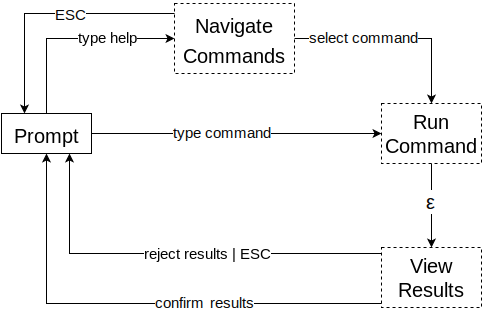
\includegraphics[width=0.8\linewidth]{figures/alternatives/undo_a.png}
  \caption{A breakdown of the procedure for undoing actions.}
  \label{fig:undoa}
\end{figure}

Figure \ref{fig:undoa} demonstrates a method which allows the user to see the
results of their actions, and then chose whether or not to carry it out.

\begin{figure}[H]
  \centering
  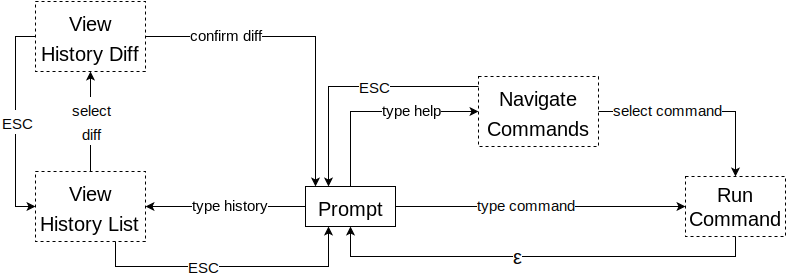
\includegraphics[width=0.8\linewidth]{figures/alternatives/undo_b.png}
  \caption{A breakdown of the procedure for undoing actions.}
  \label{fig:undob}
\end{figure}

A scheme that gives perhaps more undo ability (yet less pedagogical value) is
the ability to brows the history of your commands and the states they
represented. Figure \ref{fig:undob} shows such a scheme.

\begin{figure}[H]
  \centering
  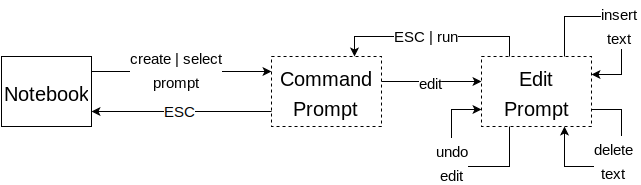
\includegraphics[width=0.8\linewidth]{figures/alternatives/undo_c.png}
  \caption{A breakdown of the procedure for undoing actions.}
  \label{fig:undoc}
\end{figure}

Another common way to deal with this problem is the style that is used by the
\emph{iPython} notebook \--- displaying the whole command history, and allowing
the user to change the text of the commands that were previously entered. Figure
\ref{fig:undoc} shows such a scheme.

\subsection{Discovery}

Users commonly want to know what they can do with given file types. We want to
provide the user with the knowledge of how to continue with their files.

\begin{figure}[H]
  \centering
  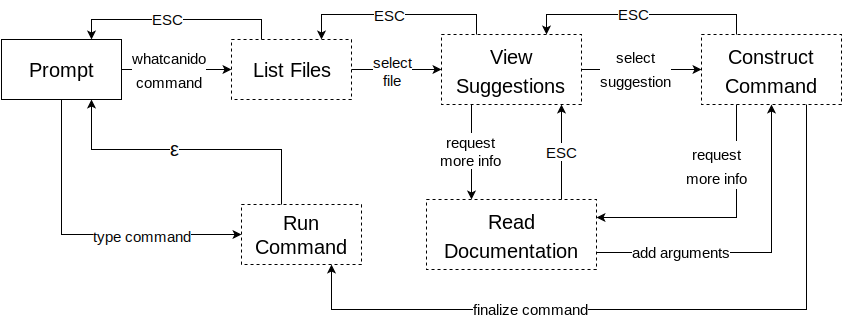
\includegraphics[width=0.8\linewidth]{figures/alternatives/file_a.png}
  \caption{A breakdown of the procedure for undoing actions.}
  \label{fig:disca}
\end{figure}

In Figure \ref{fig:disca} we present a model where first a file is selected. Once
the selection has been made, the shell can provide a list of ``what to do next''
options. This represents a more reverse polish style of shell navigation.

\begin{figure}[H]
  \centering
  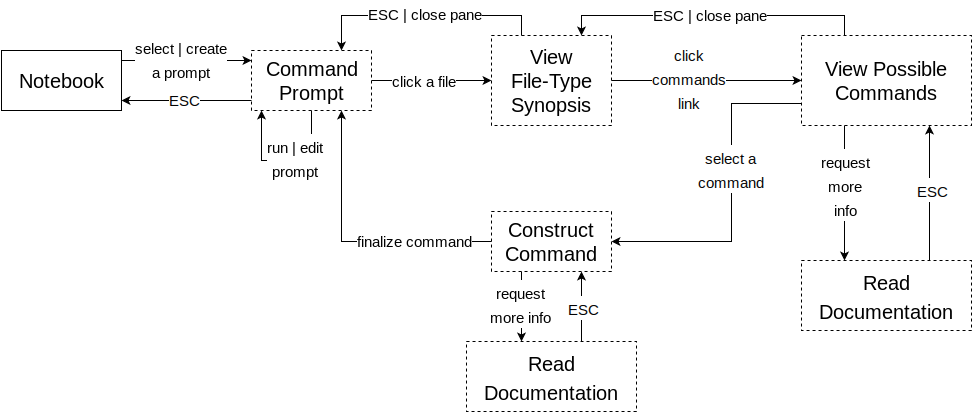
\includegraphics[width=\linewidth]{figures/alternatives/file_b.png}
  \caption{A breakdown of the procedure for undoing actions.}
  \label{fig:discb}
\end{figure}

An alternative to this, again, would be a notebook style interface, with a mouse
oriented approach. In this, we can select files, and can optionally be presented
with a list of actions.

\begin{figure}[H]
  \centering
  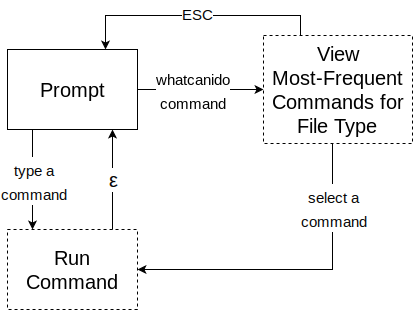
\includegraphics[width=0.8\linewidth]{figures/alternatives/file_c.png}
  \caption{A breakdown of the procedure for undoing actions.}
  \label{fig:discc}
\end{figure}

Figure \ref{fig:discc} shows the simplest way to implement this feature \--- a
special command to ask ``what is the most common task to perform on this file
type.''

\subsection{Workflow Automation}

Commonly users are performing repetitive tasks on a related set of files. They
may not understand that their workflow could be automated, or how to automate
things. The onus would then be on our software to detect common situations as
well as repetitive situations, and alert and assist the user in streamlining
their work.

\begin{figure}[H]
  \centering
  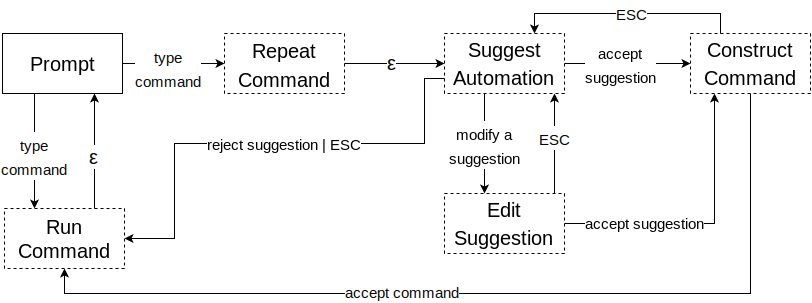
\includegraphics[width=0.8\linewidth]{figures/alternatives/automate_a.png}
  \caption{A breakdown of the procedure for undoing actions.}
  \label{fig:autoa}
\end{figure}

In Figure \ref{fig:autoa} we show perhaps the most obvious way to perform this
sort of automation \--- detect repeated commands, and suggest an automation path
(such as building a for loop). This will serve as a good, non-invasive method,
that will alert the user of features of the shell.

\begin{figure}[H]
  \centering
  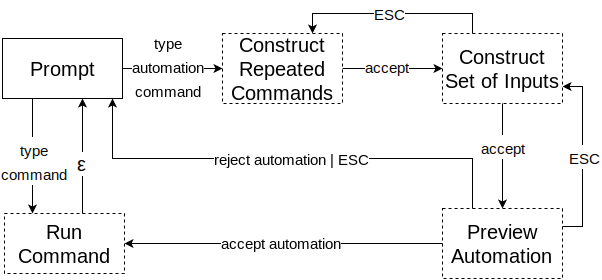
\includegraphics[width=0.8\linewidth]{figures/alternatives/automate_b.png}
  \caption{A breakdown of the procedure for undoing actions.}
  \label{fig:autob}
\end{figure}

The user, however, could be provided with an ``automate'' command, prompting
this system to provide automation suggestions. This would be an easier path to
pursue, but leave more responsibility for the user. Figure \ref{fig:autob} shows
such a scheme.

\begin{figure}[H]
  \centering
  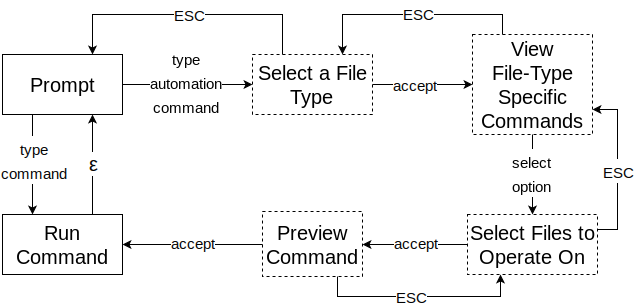
\includegraphics[width=0.8\linewidth]{figures/alternatives/automate_c.png}
  \caption{A breakdown of the procedure for undoing actions.}
  \label{fig:autoc}
\end{figure}

Finally, we could boil all automation commands down to batch processes on
related files. Figure \ref{fig:autoc} shows how the user may select related files,
and then build up a command to operate on all files.

\subsection{Preview Command}

Commonly users are not sure how what the results of their commands will be. We
feel being provided with a ``preview'' of commands may help build confidence in
the shell.

\begin{figure}[H]
  \centering
  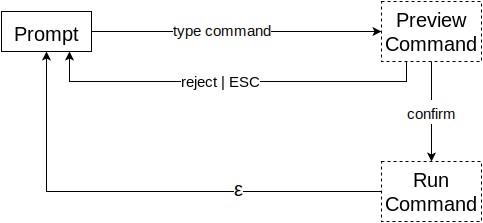
\includegraphics[width=0.8\linewidth]{figures/alternatives/preview_a.png}
  \caption{A breakdown of the procedure for undoing actions.}
  \label{fig:preva}
\end{figure}

An easy way to achieve this would be to preview the command while it is being
constructed, perhaps in the context window we have described. The user can then
fluidly work in the shell, seeing results before they occur.

\begin{figure}[H]
  \centering
  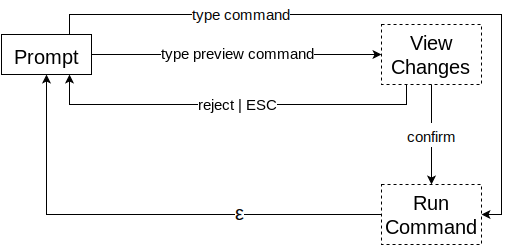
\includegraphics[width=0.8\linewidth]{figures/alternatives/preview_b.png}
  \caption{A breakdown of the procedure for undoing actions.}
  \label{fig:prevb}
\end{figure}

Figure \ref{fig:prevb} however would remove this as being the default behavior,
and allow the users to request a preview. The rest of the workflow would remain
unchanged.

\begin{figure}[H]
  \centering
  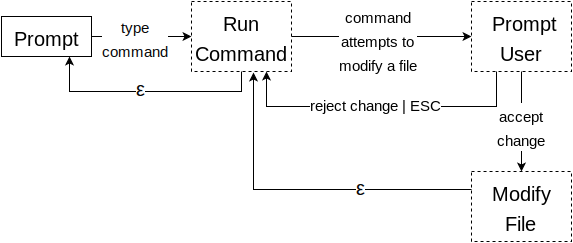
\includegraphics[width=0.8\linewidth]{figures/alternatives/preview_c.png}
  \caption{A breakdown of the procedure for undoing actions.}
  \label{fig:prevc}
\end{figure}

Finally, Figure \ref{fig:prevc} shows a case when previews are only used when
the shell detects a chance will be made to any files (probably the time when
users are most uncomfortable). This way the users are not constantly burdened
with previews, and only shown then when they really matter.

%%% Local Variables:
%%% mode: latex
%%% TeX-master: t
%%% End:
